
\begin{frame}{Learning Curves: With Transfer Learning}
    \begin{columns}
    \column{0.5\textwidth}
    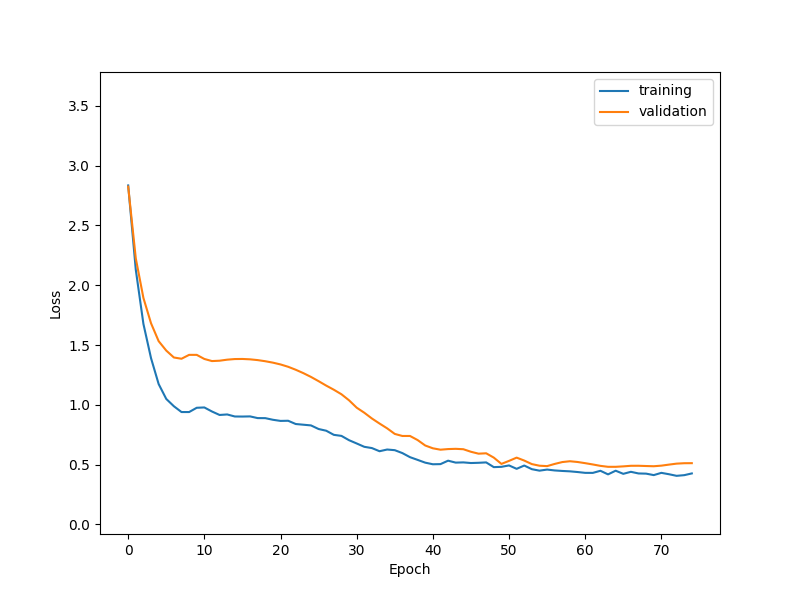
\includegraphics[height=0.8\textheight]{../project3/figures/figure1c.png}
    \column{0.5\textwidth}
    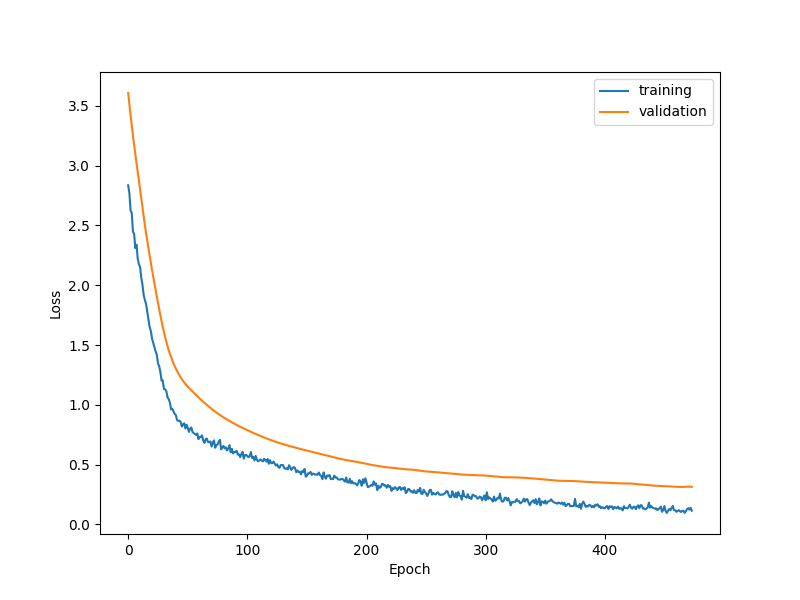
\includegraphics[height=0.8\textheight]{../project3/figures/figure1d.png}
    \end{columns}
    
    \textit{The effect of transfer learning on limited training samples}
    \begin{itemize}
        \item \textit{Left: fine-tuning; right: layer freezing}
    \end{itemize}
    \end{frame}
    
    \begin{frame}{Experimental Setup}
    \begin{itemize}
        \item \textbf{Source domain}: VA contract with specific features/parameters
        \item \textbf{Target domain}: New VA contract or same contract with different features
        \item \textbf{Architecture}: LSTM-based metamodel
        \item \textbf{Transfer approach}: Pre-trained weights from source model
    \end{itemize}
    \end{frame}
    
    \begin{frame}{Learning Dynamic Lapse}
    \textbf{The Effect of Similarity between Source and Target}
    \end{frame}
    
    \begin{frame}{Learning Curves: Learning Dynamic Lapse}
    \begin{columns}
    \column{0.5\textwidth}
    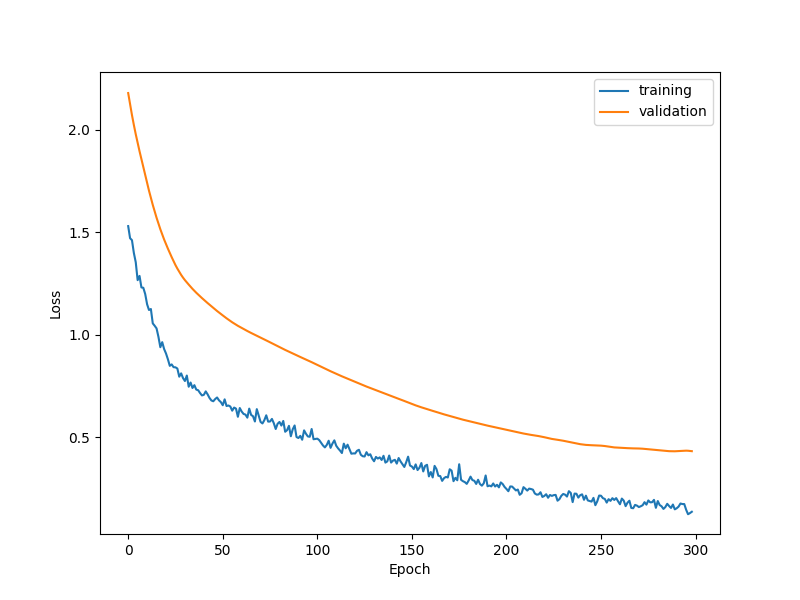
\includegraphics[height=0.8\textheight]{../project3/figures/figure2a.png}
    \column{0.5\textwidth}
    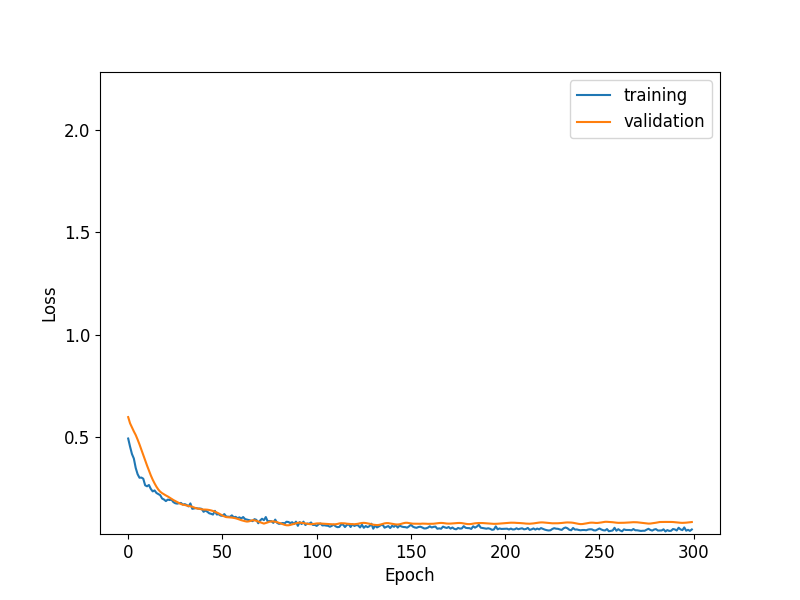
\includegraphics[height=0.8\textheight]{../project3/figures/figure2b.png}
    \end{columns}
    
    \textit{The effect of similarity between source and target on the convergence speed}
    \begin{itemize}
        \item \textit{Left: from No Lapse; right: from Static Lapse}
    \end{itemize}
    \end{frame}
    
    \begin{frame}{Results: Accuracy Comparison}
    \begin{table}
    \begin{tabular}{lcccc}
    \toprule
    \textbf{Lapse Type} & \textbf{Extensive} & \textbf{Fine-tuning} & \textbf{Layer Freezing} & \textbf{Without TL} \\
    \midrule
    No Lapse & N/A & 0.4894 & \textbf{0.3361} & N/A \\
    Static Lapse & N/A & 0.0794 & 0.0763 & N/A \\
    Dynamic Lapse & \textbf{0.0587} & N/A & N/A & \textbf{0.2950} \\
    \bottomrule
    \end{tabular}
    \end{table}
    
    \textit{Comparison of different TL methods on GMMB contracts (best MSE values)}
    \end{frame}
    
    \begin{frame}{Learning Curves: Effect of Similarity}
    \begin{columns}
    \column{0.5\textwidth}
    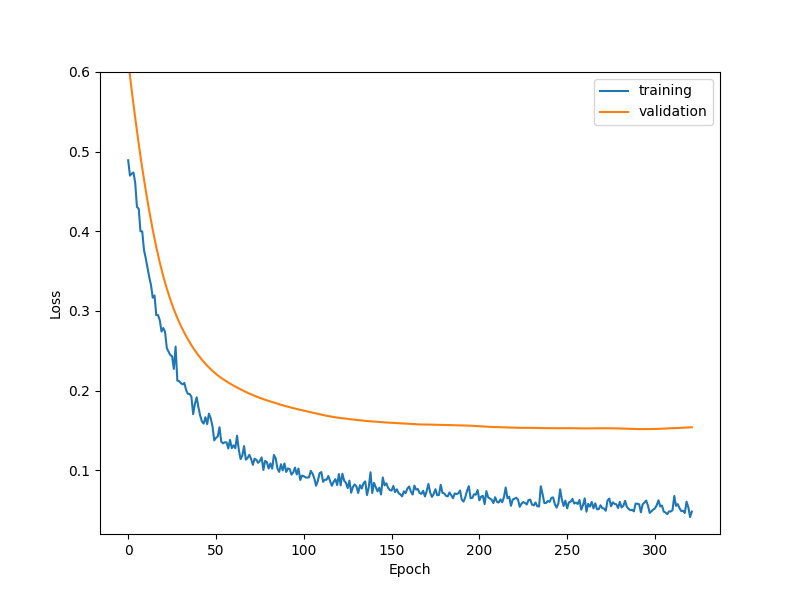
\includegraphics[height=0.8\textheight]{../project3/figures/figure3a.png}
    \column{0.5\textwidth}
    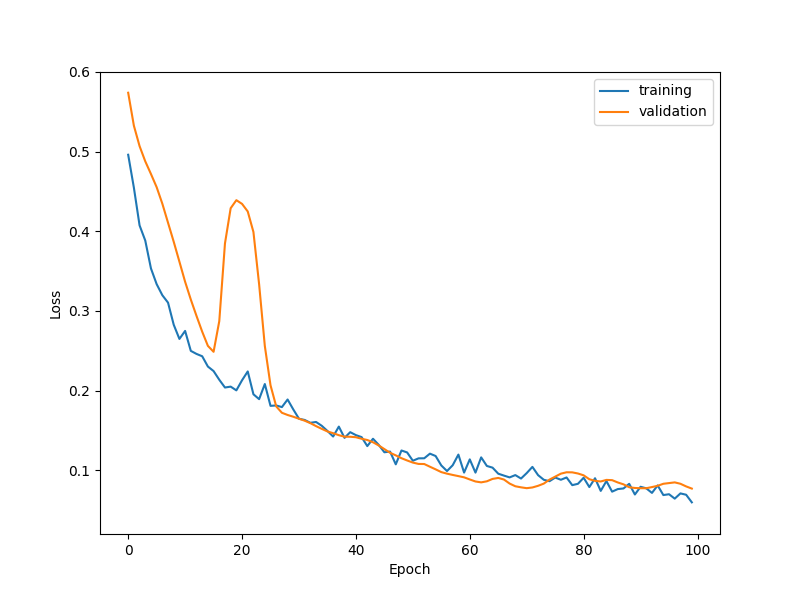
\includegraphics[height=0.8\textheight]{../project3/figures/figure3b.png}
    \end{columns}
    
    \textit{The effect of similarity between source and target on the convergence speed}
    \begin{itemize}
        \item \textit{Left: from No Lapse; right: from Static Lapse}
    \end{itemize}
    \end{frame}
    
    \begin{frame}{Transfer Knowledge to other Contract Types}
    \textbf{From GMMB to GMWB Contract}
    \end{frame}
    
    \begin{frame}{Learning Curves: Transfer Knowledge to other Contract Types}
    \begin{columns}
    \column{0.5\textwidth}
    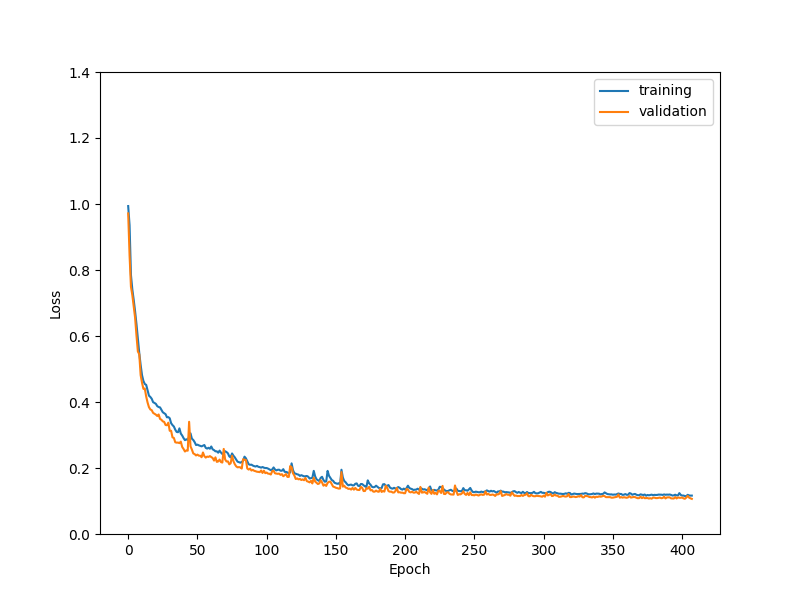
\includegraphics[height=0.8\textheight]{../project3/figures/figure4a.png}
    \column{0.5\textwidth}
    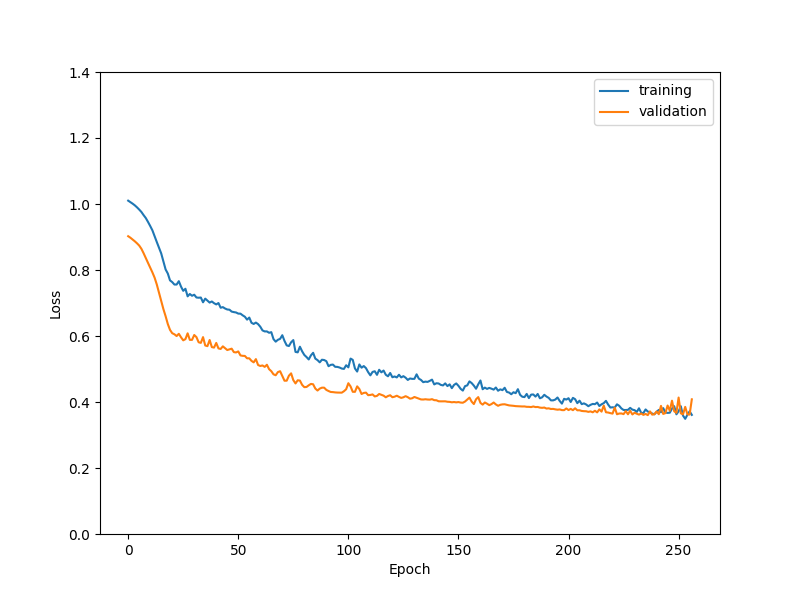
\includegraphics[height=0.8\textheight]{../project3/figures/figure4b.png}
    \end{columns}
    
    \textit{Learning curves of GMWB contracts}
    \begin{itemize}
        \item \textit{Left: 50000 samples; right: 2000 samples}
    \end{itemize}
    \end{frame}
    
    \begin{frame}{Learning Curves: Effect of Similarity}
    \begin{columns}
    \column{0.5\textwidth}
    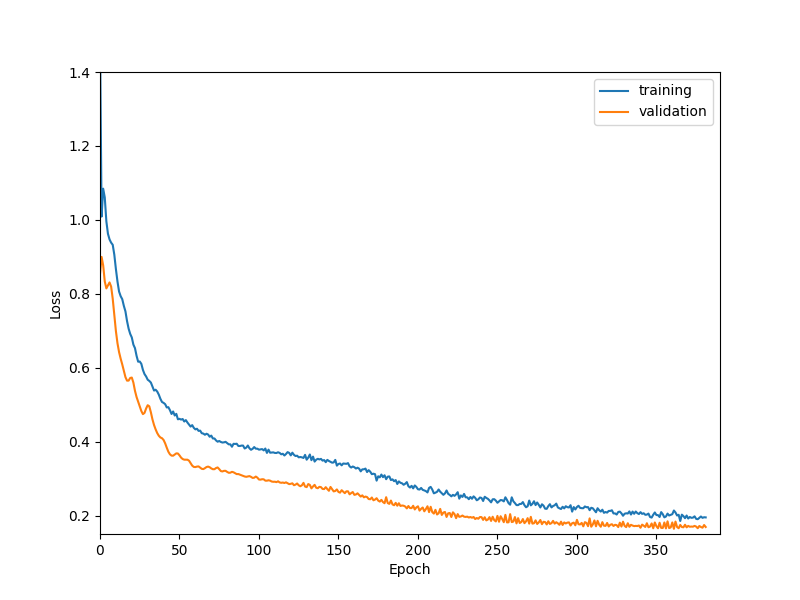
\includegraphics[height=0.8\textheight]{../project3/figures/figure4c.png}
    \column{0.5\textwidth}
    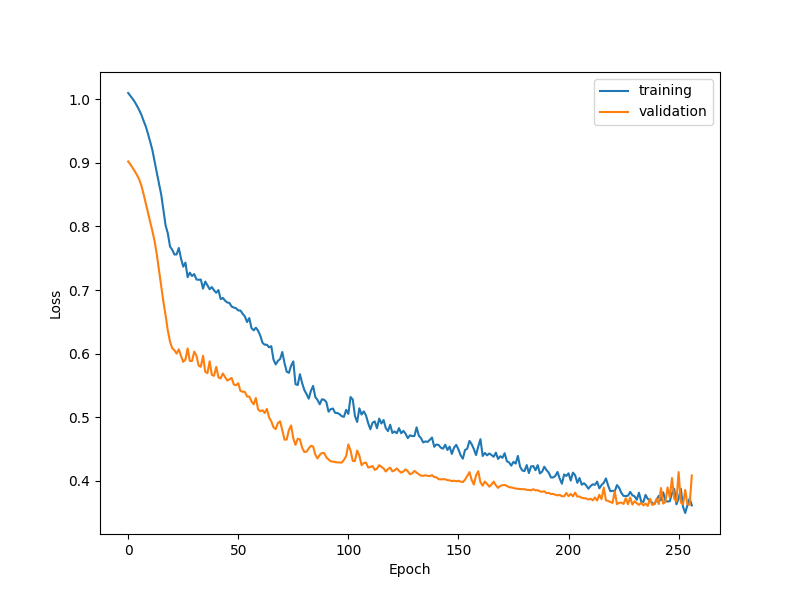
\includegraphics[height=0.8\textheight]{../project3/figures/figure4d.png}
    \end{columns}
    
    \textit{Comparison of different TL methods on GMWB contracts}
    \begin{itemize}
        \item \textit{Left: fine-tuning; right: layer freezing}
    \end{itemize}
    \end{frame}
    
    \begin{frame}{Performance Comparison (GMMB → GMWB)}
    \begin{table}
    \begin{tabular}{lcc}
    \toprule
    \textbf{Model} & \textbf{Training MSE} & \textbf{True MSE} \\
    \midrule
    Without TL & 0.3588 & 0.4188 \\
    Fine Tuning & 0.1690 & 0.1780 \\
    Layer Freezing & 0.1828 & 0.2295 \\
    Extensive Training & 0.0853 & 0.0726 \\
    \bottomrule
    \end{tabular}
    \end{table}
    
    \begin{itemize}
        \item Fine-tuning outperforms layer freezing for dissimilar tasks
        \item Both TL methods better than training from scratch
        \item Extensive training still superior with abundant data
    \end{itemize}
    \end{frame}
    
    \begin{frame}{Practical Implementation}
    \begin{itemize}
        \item \textbf{Framework}: TensorFlow/PyTorch implementation
        \item \textbf{Workflow}:
        \begin{enumerate}
            \item Train base model on source contract
            \item Freeze early layers
            \item Fine-tune later layers on target contract
            \item Deploy for production use
        \end{enumerate}
    \end{itemize}
    
    \textbf{PyTorch} is recommended.
    \begin{itemize}
        \item It is more flexible and easier to customize
        \item It is more intuitive and easier to understand 
        \item It is more efficient and easier to debug
    \end{itemize}
    \end{frame}
    
    \begin{frame}{Multi-task Learning}
    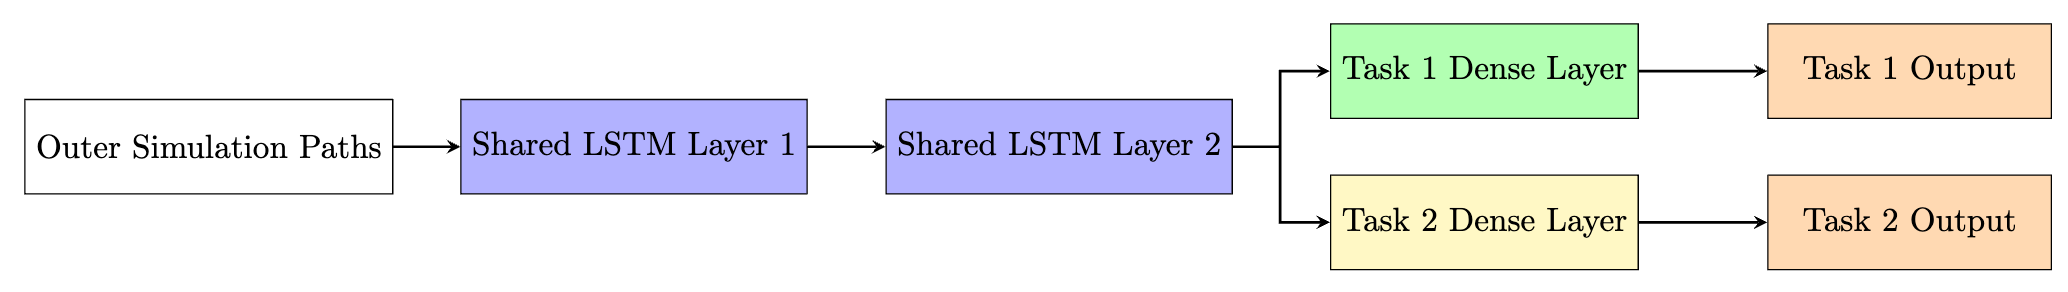
\includegraphics[width=0.9\textwidth]{../project3/figures/mtl.png}
    
    \begin{itemize}
        \item LSTM layers shared across multiple tasks
        \item Task-specific fully connected layers
        \item Objective: Minimize sum of loss functions across all tasks
    \end{itemize}
    \end{frame}
    
    \begin{frame}{Multi-task Learning Framework}
    \textbf{Input}: Set of $K$ tasks $\{\mathcal{T}_k\}_{k=1}^K$ with datasets $\mathcal{D}_k = \{(X_k^{(i)}, L_k^{(i)})\}_{i=1}^{M_k}$, shared parameters $\theta_0$, and task-specific parameters $\theta_k$ for each task $k$
      
    \textbf{Algorithm}:
    \begin{enumerate}
        \item Train the multi-head LSTM metamodel on all $K$ tasks simultaneously by minimizing the multi-task loss function:
        \begin{equation}
            \min_{\theta_0, \{\theta_k\}_{k=1}^K} \sum_{k=1}^K \frac{1}{M_k} \sum_{i=1}^{M_k} \left( f_i(X_k^{(i)}; \theta_0, \theta_k) - L_k^{(i)} \right)^2
        \end{equation}
        \item Update both the shared parameters $\theta_0$ and task-specific parameters $\{\theta_k\}_{k=1}^K$ simultaneously using backpropagation and gradient descent with learning rate $\alpha$
    \end{enumerate}
    
    \textbf{Output}: Trained multi-task LSTM metamodel $f(\cdot; \theta_0, \{\theta_k\}_{k=1}^K)$ for all $K$ tasks
    \end{frame}
    
    \begin{frame}{Multi-task Learning: GMMB and GMWB}
    \begin{columns}
    \column{0.5\textwidth}
    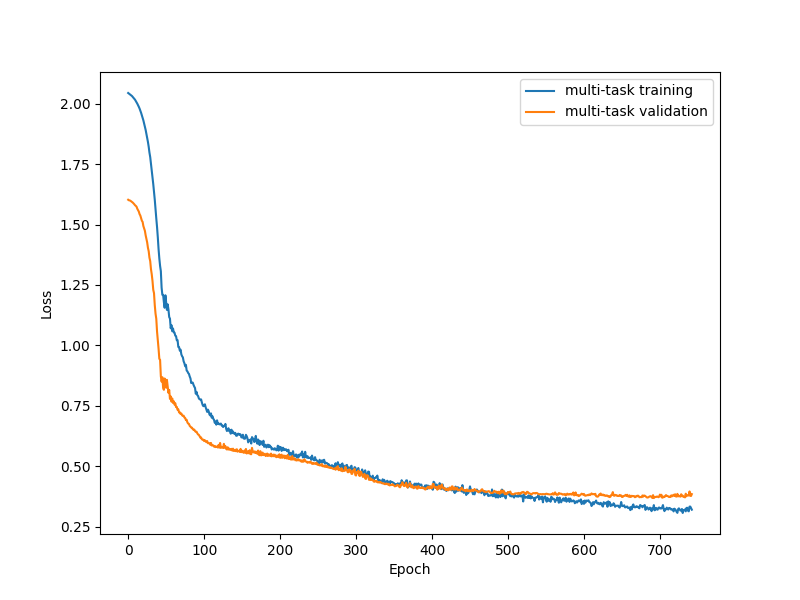
\includegraphics[height=0.8\textheight]{../project3/figures/figure5a.png}
    \column{0.5\textwidth}
    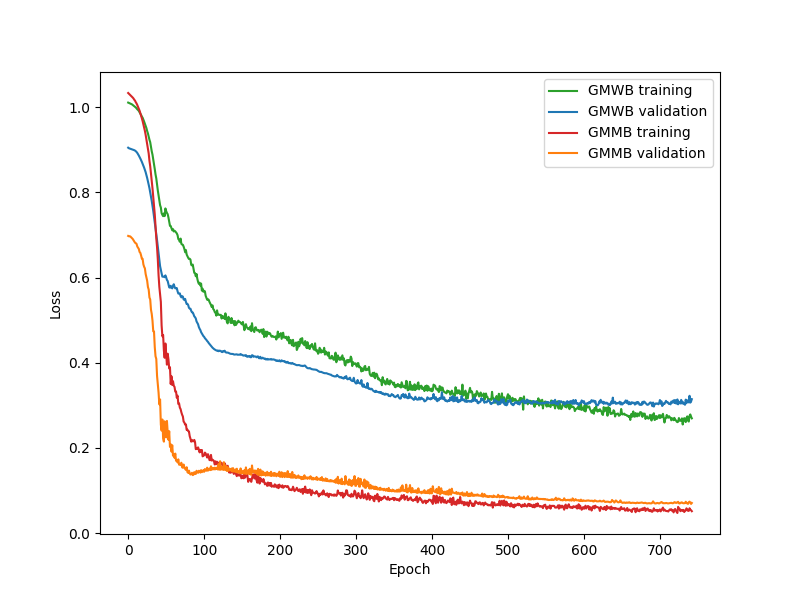
\includegraphics[height=0.8\textheight]{../project3/figures/figure5b.png}
    \end{columns}
    
    \textit{Multi-task learning of GMMB and GMWB}
    \begin{itemize}
        \item \textit{Left: total MSE; right: individual MSE}
    \end{itemize}
    \end{frame}
    
    \begin{frame}{Multi-task Learning: GMMB and GMWB}
    \begin{columns}
    \column{0.5\textwidth}
    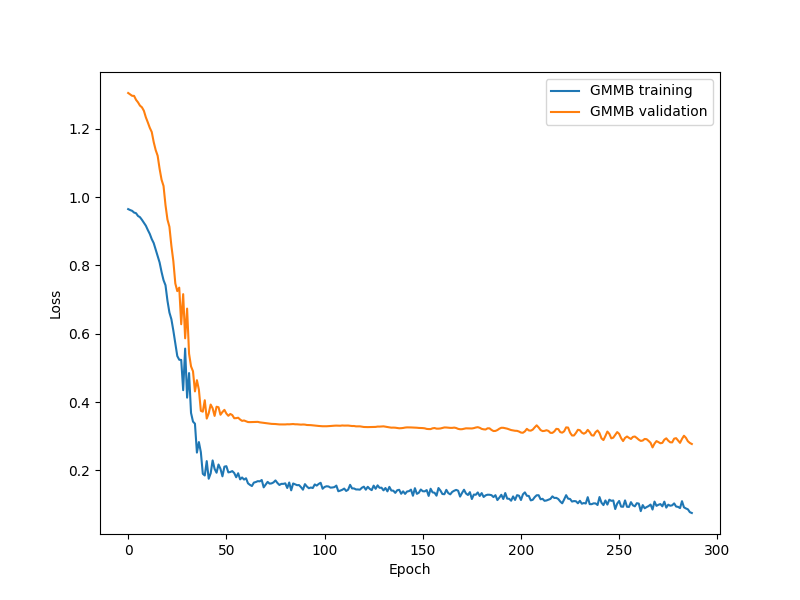
\includegraphics[height=0.8\textheight]{../project3/figures/figure5c.png}
    \column{0.5\textwidth}
    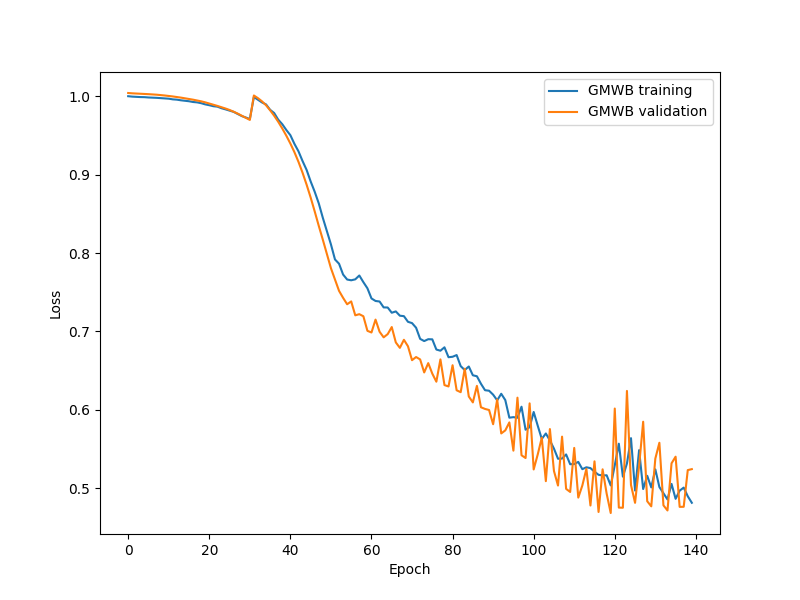
\includegraphics[height=0.8\textheight]{../project3/figures/figure5d.png}
    \end{columns}
    
    \textit{Training without multi-task learning}
    \begin{itemize}
        \item \textit{Left: GMMB; right: GMWB}
    \end{itemize}
    \end{frame}
    
    \begin{frame}{Challenges \& Limitations}
    \begin{itemize}
        \item Determining optimal layer freezing strategy
        \item Handling significantly different contract structures
        \item Quantifying uncertainty in transfer learning predictions
        \item Regulatory acceptance of black-box approaches
    \end{itemize}
    \end{frame}
    
    \begin{frame}{Conclusions}
    \begin{itemize}
        \item Transfer learning significantly improves metamodeling for VA contracts:
        \begin{itemize}
            \item Faster training convergence
            \item Better prediction accuracy
            \item Reduced computational requirements
        \end{itemize}
        \item Enables more frequent risk assessments and faster decision-making
    \end{itemize}
    \end{frame}
    
    \begin{frame}{Future Directions}
    \begin{itemize}
        \item Incorporating domain knowledge into transfer process
        \item Extension to other insurance and financial products
        \item Multi-task learning with more than two tasks
    \end{itemize}
    \end{frame}
